\documentclass{article}

\usepackage{booktabs}
\usepackage{tikz}
\usepackage{logicproof}
\usepackage[capitalize,noabbrev]{cleveref}

\title{Logic Homework 1}
\author{Name\\s1234567}

\begin{document}

\maketitle

This document is a template for the homework assignments.
It includes all packages necessary to produce truth tables, parse trees, proofs, and semantic tableaux.

\section*{Question 1}
\paragraph{a)}

The following proof shows the validity of the sequent $(p \lor q) \lor r \vdash p \lor (q \lor r)$, as shown in Example 1.17 on page 18 of [HR04].

\begin{logicproof}{2}
    (p \lor q) \lor r & premise \\
    \begin{subproof}
        (p \lor q) & assumption \\
        \begin{subproof}
            p & assumption \\
            p \lor (q \lor r) & $\lor\mathrm{i}_1$, 3
        \end{subproof}
        \begin{subproof}
            q & assumption \\
            q \lor r & $\lor\mathrm{i}_1$, 5 \\
            p \lor (q \lor r) & $\lor\mathrm{i}_2$, 6
        \end{subproof}
        p \lor (q \lor r) & $\lor$e, 2, 3--4, 5--7
    \end{subproof}
    \begin{subproof}
        r & assumption\\
        q \lor r & $\lor\mathrm{i}_2$, 9 \\
        p \lor (q \lor r) & $\lor\mathrm{i}_2$, 10
    \end{subproof}
    p \lor (q \lor r) & $\lor$e, 1, 2--8, 9--11
\end{logicproof}

\cref{mytable} shows the truth table of $(p \to \neg q) \to (q \lor \neg p)$ and all of its subformulas, as shown in Figure 1.8 on page 40 of [HR04].

\begin{table}[ht]
    \centering
    \begin{tabular}[t]{ccccccc} 
        \toprule
        \rotatebox{90}{$p$}     & \rotatebox{90}{$q$}     & \rotatebox{90}{$\neg p$} & \rotatebox{90}{$\neg q$} & \rotatebox{90}{$p \to \neg q$} & \rotatebox{90}{$q \lor \neg p$} & \rotatebox{90}{$(p \to \neg q) \to (q \lor \neg p)$} \\
        \midrule
        {\tt T} & {\tt T} & {\tt F}  & {\tt F}  & {\tt T}        & {\tt T}         & {\tt T} \\
        {\tt T} & {\tt F} & {\tt F}  & {\tt T}  & {\tt T}        & {\tt F}         & {\tt F} \\
        {\tt F} & {\tt T} & {\tt T}  & {\tt F}  & {\tt F}        & {\tt T}         & {\tt T} \\
        {\tt F} & {\tt F} & {\tt T}  & {\tt T}  & {\tt T}        & {\tt T}         & {\tt T} \\
        \bottomrule
    \end{tabular}
    \caption{An example of a truth table for a more complex logical formula.}
    \label{mytable} 
\end{table}

\cref{mytree} shows the parse tree of $(((\neg p) \land q) \to (p \land (q \lor ( \neg r))))$, as shown in Figure 1.3 on page 34 of [HR04]. 

\begin{figure}[ht]
    \centering
    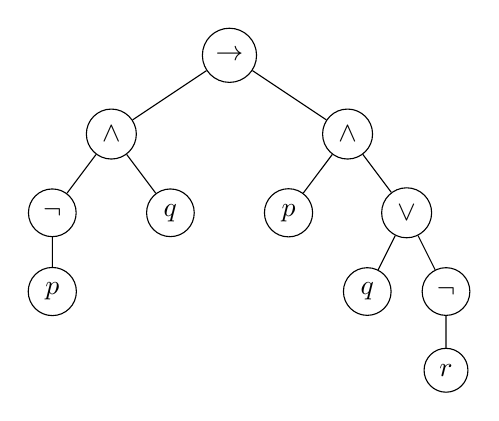
\begin{tikzpicture}[
        every node/.style={circle,draw},
        level/.style={sibling distance = 3cm/#1,level distance = 1.0cm}]
    \node {$\to$} 
        child { node {$\land$} 
            child { node {$\lnot$} 
                child { node {$p$} }
            }
            child { node {$q$} }
        }
        child { node {$\wedge$} 
            child { node {$p$} }
            child { node {$\vee$} 
                child { node {$q$} }
                child { node {$\neg$} 
                    child { node {$r$} }
                }
            }
        }
        ;
    \end{tikzpicture}
    \caption{A parse tree representing a well-formed formula.}
    \label{mytree}
\end{figure}

\cref{mytableau} shows the semantic tableau from Voorbeeld 3.7 on page 40 of [BDKLM03].

\begin{figure}[ht]
    \centering
    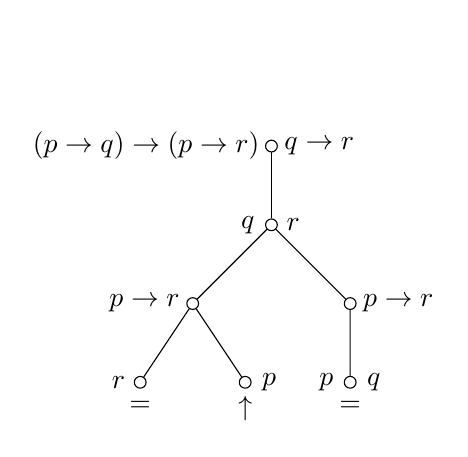
\begin{tikzpicture}[
        every node/.style={circle,draw,inner sep=1.5pt},
        level/.style={sibling distance = 4cm/#1,level distance = 1.0cm}]
        \node [label={left:$(p \to q) \to (p \to r)$},label={right:$q \to r$}] {} 
            child { node [label={left:$q$},label={right:$r$}] {} 
                child { node [label={left:$p \to r$}] {} 
                    child { node [label={left:$r$},label={below:$=$}] {} }
                    child { node [label={right:$p$},label={below:$\uparrow$}] {} }
                }
                child { node [label={right:$p \to r$}] {} 
                    child { node [label={left:$p$},label={right:$q$},label={below:$=$}] {} }
                }
            }
            ;
    \end{tikzpicture}
    \caption{A semantic tableau with two closed branches (indicated by double lines) an open branch (indicated by an arrow).}
    \label{mytableau}
\end{figure}

\end{document}